\documentclass[11pt]{article}
\usepackage{graphicx}
\usepackage{hyperref}
\hypersetup{
    colorlinks=true,
    linkcolor=blue,
}
\usepackage[margin=1in]{geometry}
\linespread{1.2}

\title{Political Economy of Social Assistance in the Justice and Development Party (AKP) Era}
\author{Alper Yıldırım}
\date{}

\begin{document}
\maketitle

\begin{abstract}
\textit{In February 2001, Turkey had experienced a severe economic crisis that had wide-scale impacts on the Turkish economy, such as income distribution, banking sector, and the declines in output and unemployment. After the crisis, the Turkish economy had faced a neoliberal restructuring through the EU membership process and the IMF program. On the other hand, the Justice and Development Party (AKP) came into power in 2002 and has been the governing party since then. Therefore, in the neoliberal restructuring process of Turkey, AKP was the governing party and thusly the party executed economic and social transformations. One important aspect of that transformation is the changes in social assistance programs, since AKP paid attention to the social assistance and reformed certain aspects of the social security system. This paper aims to examine the changes of social assistance system during the AKP rule from a political economy perspective and to mark certain historical breakdown in social assistance using quantitative data provided by the World Bank API. The most striking finding of this research is the changing attitude in social assistance in Turkey after 2008 Global Financial Crisis regarding the urban/rural distributions of social assistance and the average per capita shares of different income quantiles from the social assistance.}

\end{abstract}

\section{Introduction}

In February 2001, Turkey had experienced a severe economic crisis that had wide-scale impacts on the Turkish economy, such as income distribution, banking sector, and the declines in output and unemployment. As a consequence of the economic crisis, the Turkish economy’s restructuring process had started in which the new political actors, the IMF and World Bank, and the EU membership process were influential determinants \cite{onics2009beyond}. As most authors claimed, what Turkey had experienced is the neoliberal way of restructuring with an IMF-led program \cite{yeldan2006neoliberal}. Meanwhile, the Justice and Development Party (AKP) overwhelmingly won the election in November 2002 and has been the ruling party in Turkey since 2002. Considering the rise of the AKP government with the Turkish economy’s significant changes after 2001, the AKP governments have witnessed and directed some remarkable economic and social transformations of Turkey. \\

\noindent In the AKP era, the transformation of the social assistance had been a substantial part of the electoral strategy of the AKP, and that phenomenon was examined alongside with the restructuring of the Turkish economy by scholars \cite{buugra2006turkish, elveren2008social, yoruk2020electoral}. AKP won the general elections in 2002, 2007, 2011, 2015, and 2018 which corresponds a wide time range and—if local elections and presidency elections are included—too many elections. Furthermore, during the AKP rule, 2008 Global Financial Crisis had been experienced. The role of 2008 Global Financial Crisis and the influence of the elections on the social assistance spendings can be observed and examined through the quantitative data. Yet, in order to have a better understanding of the political economy of social assistance in the AKP era, the non-public welfare provision and the transformation of social assistance from a historical perspective are needed. This paper aims to examine the political economy of social assistance policies in the AKP era—including non-public welfare actors, e.g., Göçmen’s \cite{goccmen2014religion, goccmen2018non} examination of religiously motivated organizations—while discussing the previous economic and sociological work on social assistance. The quantitative data for this research will be provided through the World Bank Indicators API, and thusly, the social assistance policies of the AKP will be examined.

\section{Literature Review}

\noindent Yeldan, in his paper, had worked on 2001 crisis of Turkey while focusing on the role IMF and neoliberalization. First of all, Yeldan had listed the characteristics of the neoliberal agenda for the emerging and developing markets such as flexible labor markets, financial deregulation, flexible exchange rate regimes, etc. \cite{yeldan2006neoliberal}. While Yeldan examined the pre-2001 conditions that forced Turkey to 2001 crisis, for the purpose of this study, the post-2001 effects have priority. Yeldan propounded that the crisis administration led by the IMF was worked as a debt management program which make Turkish economy later on dependent on short-term foreign finance with relatively higher interest rates. At the end, Yeldan was critical to the new economic environment created after the 2001 crisis. For Yeldan, that in the new financial environment, Turkey became more volatile to “the speculative caprices of financial arbiters” which make him to question the sustainability of growth performance for Turkey \cite{yeldan2006neoliberal}. Öniş also focused on the structural changes in Turkish economy and the institutional reforms after the 2001 crisis. In this study, Öniş underlined the commitment of the AKP to the IMF programs and the EU membership process in that way that their impact on the confidence of domestic and foreign capital for the recovery process of Turkey \cite{onics2009beyond}. However, according to Öniş, there was no significant progress in the issue of income inequality of Turkey after 2001, similar to pre-2001 neoliberalization model. Yet, Öniş admitted that the low-income groups supported the AKP in the electoral politics, even though the labor groups were critical of the recovery after 2001 because of its unequal nature \cite{onics2009beyond}. In his paper, Öniş compared some important economic indicators’ pre-2001 and post-2001 levels to evaluate the consequences of the recovery process (2009). The most striking changes in Turkish economy in Öniş’s comparison are the reduce in the budget deficits of Turkey from the very large levels to the IMF target and Maastricht requirements levels, the reduce in the ratio of debt to Gross National Product, and the inflation data from chronically high and unstable levels to the single digit levels \cite{onics2009beyond}. \\

\pagebreak

\noindent Buğra and Keyder, two prominent scholars of the field, had worked on the transformation of the welfare regime in Turkey in an early period of the AKP rule. First of all, the authors pointed out that in the earlier regime of welfare of Turkey was based on the formally employed people with “the corporatist lines” \cite{buugra2006turkish}. However, as the share of urban population has increased and informal economy has grown, the former welfare regime became more limited. Buğra and Keyder frankly stated that “[…] dependency ratios increased as the workers in the informal sector did not contribute to social security funds but benefited as dependents of a family member who did” (\cite{buugra2006turkish}. Therefore, similar to most countries’ old-age pension systems after 1980 period, the financial sustainability of social assistance spendings got harder. In the section on pensions, Buğra and Keyder underlined that the sustainability problems in the pension system was not caused by the ageing of population but the populist policies of 1990s \cite{buugra2006turkish}. In another study focusing on pension reforms in Greece and Turkey, Güleç did not stress populist policies of the past, rather she underlined the fact that structural adjustment programmes and EU membership conditionalities had forced both Turkey and Greece to reform their pension systems \cite{gulecc2014politics}. Thereafter, Buğra and Keyder examined the health system of Turkey in its transformation. The authors appreciated the ongoing reform process, since the previous health system of Turkey was depending on the employment status which both decreased coverage rate and increased financial burden of health system. The petty producers and self-employed population were among the most negatively influenced groups, since they have limited power to qualify for a Green Card in the previous system \cite{buugra2006turkish}. Lastly, another striking argument of Buğra and Keyder is that employment based social security coverages forced the people who have not enrolled in formal economy to rely on their family members and kinship ties, and most importantly, “other informal relations of reciprocity, which can also involve clientelistic relations with political authorities” \cite{buugra2006turkish}. The study of Buğra and Keyder, even though it is a very early study of the AKP rule, offers enormous insights to understand social security policies in Turkey. \\

\noindent In their study, Yörük and Comin had examined the rule of AKP in Turkey and Partido dos Trabalhadores (PT) in Brazil based on their strategies relying on “the poor”. The authors claimed that the neoliberal re-organization of the economies of these countries created an obstacle to form multi-class alliances for elections. Therefore, for the sake of electoral success, AKP and PT operationalized the social assistance polices to “the poor” \cite{yoruk2020electoral}. At that point, Yörük and Comin mentioned “the new welfare state” in the context of the emerging markets. Their finding is compatible with the assertion of Piven and Minnite that while welfare retrenchments are observable in the advanced capitalist countries, the welfare regimes based on their social assistance policies expanded in the developing markets \cite{yoruk2020electoral, pivenminnite:2015}. In a more recent paper, Bargu and Yörük underlined that non-contributory social assistance programs instead of the contributory social policies are more prominent in countries where the informal employment is in high level \cite{yorukbargu:2021}. \\

\noindent Lastly, Göçmen had worked on the role of religiously motivated associations (RMAs) on the welfare regime. For Göçmen, the prevalence of the religiously motivated associations in the non-public welfare area in the last two decades is not related to the retrenchments within the welfare state of Turkey and that assertion is compatible with Yörük and Comin’s claim on the new welfare state in the emerging markets \cite{goccmen2014religion}. So, Göçmen claimed that while economic neoliberalization after the coup d’état of 1980 had increased the demand for social assistance and as the Welfare Party, MUSIAD, Deniz Feneri, or similar instances demonstrated that the religion became more central in the political economy of Turkey after 1980 \cite{goccmen2014religion}. Even though the reforms of Turkish social policy made improvement in the system, the prominence of the religiously motivated associations has increased. Therefore, at the end, Göçmen concluded that the best way to understand that prominence of RMAs is not the welfare retrenchments, but the political environments and social conditions since the 1980s. Later on, Göçmen has revisited the study of religiously motivated associations as non-public welfare actors in a comparative perspective in a qualitative research. In this later study, Göçmen had asserted some remarkable claims such that religiously motivated associations became the main actors of the welfare provisioning, and they became more politicized along with the AKP regime. Therefore, those became the main actors in the welfare provision are the religiously motivated associations that have ties to the AKP \cite{goccmen2018non}. Thusly, in the non-public welfare provision, the patronage and cronyism had become obvious in the AKP rule.

\section{Data}

\noindent The social assistance data for Turkey was derived from the World Bank database. In order to compile necessary data for this study, the World Bank Indicators API (Application Programming Interface) was operationalized using Python programming language. All the visualizations were prepared in Python using \verb|Matplotlib| module. First of all, average per capita transfer for all social assistance data was scraped based on 6 different levels: the average level, and for each income quantile separately. In the World Bank documentation, it is stated that this indicator is “the average transfer amount of social protection and labor programs among beneficiaries”. Thereafter, the data of the coverage of all social assistance was derived from World Bank API again. The coverage data was also compiled in three different levels: the average level, the urban average, and the rural average. The World Bank documentation stated that as a definition of that indicator, “percentage of population participating in social protection and labor programs” and both indirect and direct benefits were contained in this dataset. Both average per capita of social assistance and the coverage of social assistance data were compiled and represented in a time-series graph. Lastly, the coverage rate of social pensions data was scraped through the World Bank Indicators API which variable signifies the percentage of each income quantile “participating in social protection and labor programs” for social pensions. The output for each variable is presented in Figure \ref{fig:avgtr}, Figure \ref{fig:cvrg}, and Figure \ref{fig:pnsn}.

\section{Results}

\noindent As Figure \ref{fig:avgtr} demonstrated, the average per capita transfers for all social assistance had rapidly increased after the 2008 Global Financial Crisis. Especially for the 4th and 5th income quantiles which groups actually have more income than the other quantiles have begun to receive more per capita transfer from the social assistance system. The results seem odd, however, the data of the number of social assistance beneficiaries for different income quantiles may help to figure out that trend. However, that data was available neither in Turkstat nor World Bank Indicators API. After the 2008 Global Financial Crisis period, another observable trend is the convergence between the different income quantiles after 2015. As the average per capita transfer of 5th quantile climbed rapidly in 2008, there was a huge difference between the 5th quantile and the other income quantiles. However, since 2015, there is a trend of convergence that resulted similar average levels for each income quantiles in 2018. Yet, the 5th income quantile, which group receives more income than other quantiles, also received more average per capita assistance. If the data of the number of beneficiaries for each income quantile would be acquired, there would be an opportunity to confirm or reject the claims of Yörük and Comin \cite{yoruk2020electoral}. \\

\begin{figure}[htbp]
    \begin{center}
    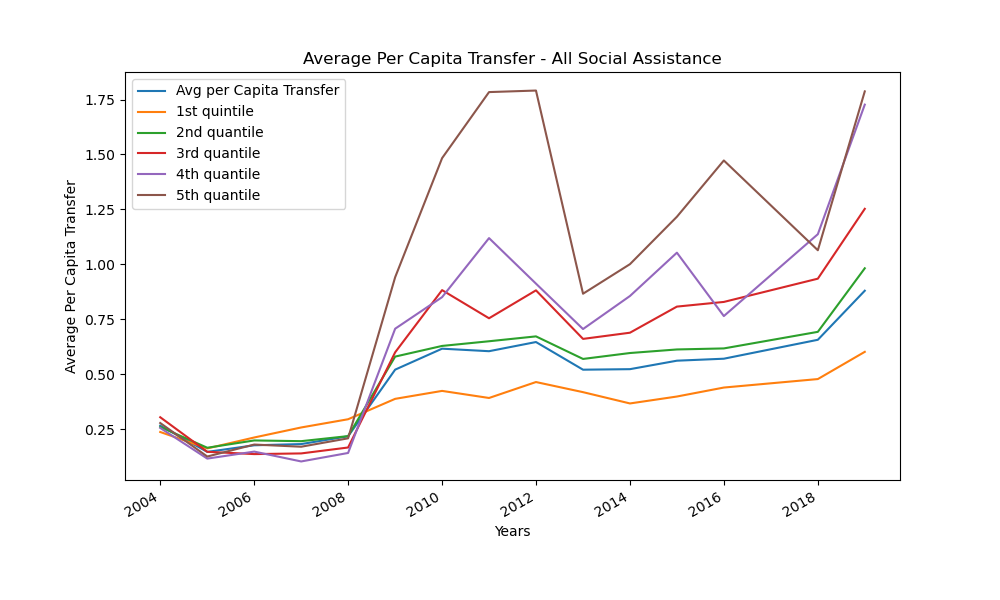
\includegraphics[width=6in]{avgpercaptransfer.png}
    \caption{Average Per Capita Transfer - All Social Assistance}
    \label{fig:avgtr}
    \end{center}
\end{figure}

\noindent On the other hand, the coverage date represented at Figure \ref{fig:cvrg} showed another trend for the 2008 Global Financial Crisis. While in the 2004-2008 time interval, the average coverage ratio has increased steadily and even reached to 35\% levels, the 2008 Crisis created a turning point. After 2008, the coverage ratio for all social assistance had decreased rapidly. The declining trend is more significant for urban areas than rural areas. In 2013, the average levels of coverage of social assistance became below 20\% level, which corresponds approximately 20\% decrease in the last 5 years. A closer look to Figure \ref{fig:cvrg} demonstrated that the coverage of social assistance in the urban areas came into the below 15\% level while the coverage in the rural areas were still around 25\% levels. However, in the pre-2008 levels of coverage, the rural and urban ratios were close to each other, and the urban coverage even slightly exceeded the rural coverage. Lastly, Figure \ref{fig:pnsn} which represent the coverage rate of social pensions did not contain any significant historical trend for different income quantiles, except the unprecented increase of the 1st quantile—the poorest quantile—in the coverage after 2016. The mixed trends in the Figure \ref{fig:pnsn} did not contribute to understand the political economy of social assistance or social security system in Turkey during the AKP rule.

\begin{figure}[htbp]
    \begin{center}
    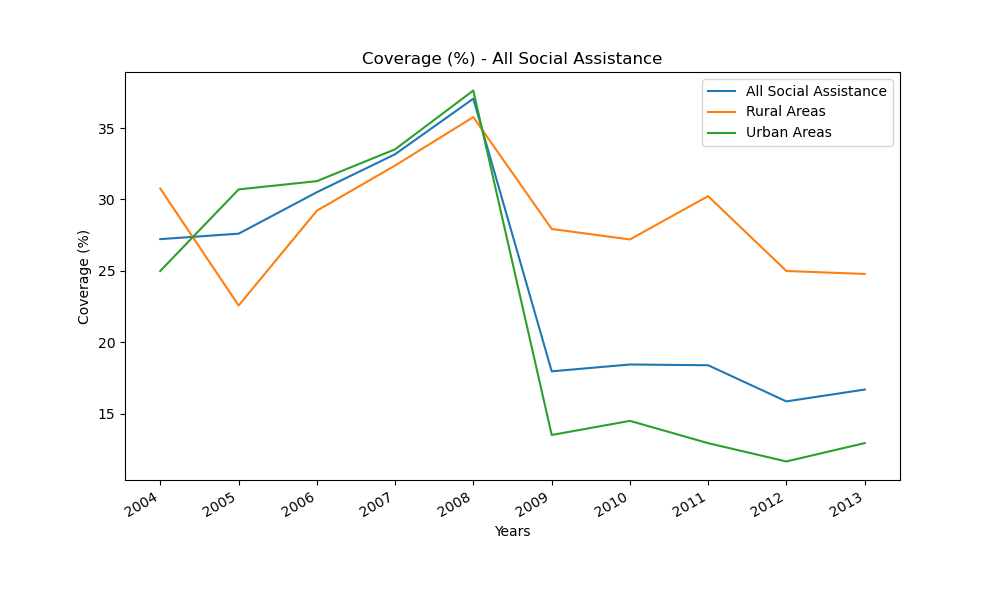
\includegraphics[width=6in]{cvrg_asst.png}
    \caption{Coverage of All Social Assistance (\%)}
    \label{fig:cvrg}
    \end{center}
\end{figure}

\section{Conclusion}

\noindent As the findings demonstrated, the only breakdown in both the coverage and average per capita transfer is the 2008 Global Financial Crisis. Therefore, the best of my knowledge, the relationship between the electoral success and social assistance spending is neither rejected nor accepted, that is what Yörük and Comin argued \cite{yoruk2020electoral}. Furthermore, since there is no data available regarding the non-public welfare actors, the role of those institutions could be confirmed only through the qualitative research, which Göçmen had accomplished \cite{goccmen2018non}. For the further studies in this field, the indicators to measure the influence of non-public welfare actors should be determined and correspondingly, the data collection process should be started. However, the findings provide some support for an argument that the rural areas became more prior for the AKP governments in regard to social assistance than urban areas. Since there is no decrease in the rate of the poorer populations of urban areas or informal employment rate in the last two decades, the prominence of the social assistance in the rural areas implied a political decision for the AKP rule. Because of the limitations in the data, the scope of this research became also limited. However, it can be fairly claimed that the elections did not influence the coverage rate or average per capita transfers in the social assistance rate directly neither in negative nor in positive way. This outcome is contrary to common belief that the coverage of social assistance was increased in every election time. This outcome confirmed the claims of Bargu and Yörük that if both electoral competition and the number of mass protests are high concurrently, the positive association with social assistance spendings is observed \cite{yorukbargu:2021}. But it should be stated that, only if the mass protests or riots occur during the time of electoral competition, their effect on social assistance spendings becomes significant, according to their study. Therefore, in the following studies, the effect of what Charles Tilly conceptualized “contentious politics”, i.e., mass protests, strikes, guerilla movements, etc., on the economic variables including the social assistance system should be further examined \cite{Tilly1988-jc}.

\begin{figure}[htbp]
    \begin{center}
    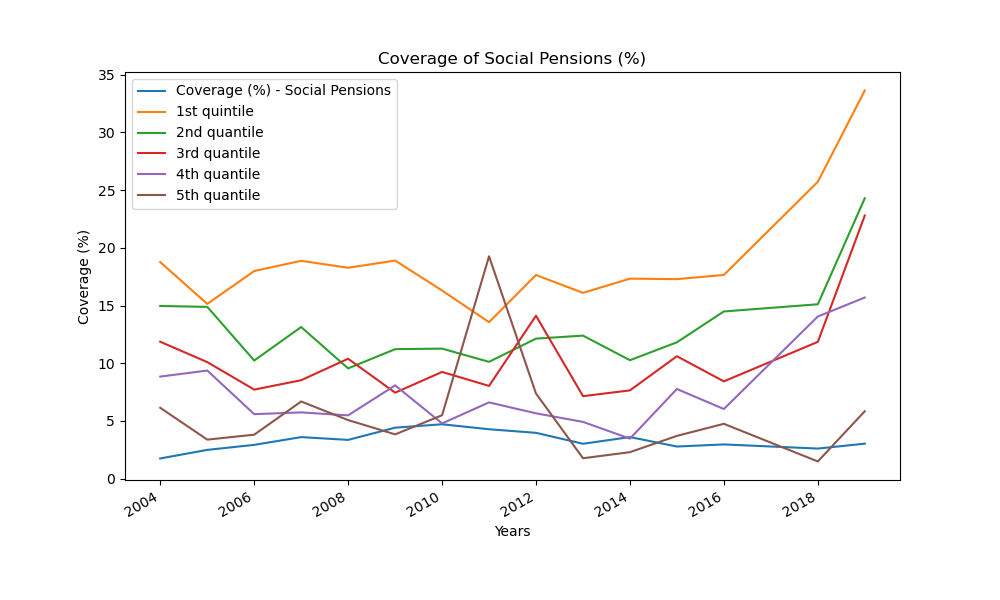
\includegraphics[width=6in]{pensioncoverage.png}
    \caption{Coverage of Social Pensions (\%)}
    \label{fig:pnsn}
    \end{center}
\end{figure}

\section*{Appendix}

The \LaTeX\;and Python scripts composed for this study could be found at \href{https://github.com/yildirimalper/tr-socialasst}{this GitHub repository}. 


\pagebreak

\bibliographystyle{abbrv}
\bibliography{references.bib}

\end{document}